% TMLR version of the paper, built with tectonic (XeTeX). Nothing needs pdfLaTeX-only features.
% Anonymous submission:  tectonic main.tex      -> main.pdf
% Named preprint:        tectonic preprint.tex  -> preprint.pdf  (preprint.tex sets \tmlrpreprint)
% Figures and tables are generated from the runs/ data: see make_figures.py and make_tables.py.
\documentclass[10pt]{article}
\ifdefined\tmlrpreprint
  \usepackage[preprint]{tmlr}
\else
  \usepackage{tmlr}
\fi

\usepackage{hyperref}
\usepackage{url}
\usepackage[protrusion=true,expansion=false]{microtype}
\usepackage{amsmath}
\usepackage{graphicx}
\usepackage{booktabs,tabularx,array}
\usepackage{xcolor}
\usepackage{etoolbox}
\AtBeginEnvironment{table}{\setlength{\belowcaptionskip}{5pt}}

\definecolor{linkblue}{HTML}{1F3A68}
\hypersetup{
  colorlinks = true,
  linkcolor  = linkblue,
  citecolor  = linkblue,
  urlcolor   = linkblue,
  pdftitle   = {Small Updates Break First: A Pre-Registered Study of Fine-Tuning Gains Under MLX and GGUF Quantization},
  pdfkeywords = {quantization, LoRA, fine-tuning, MLX, GGUF, pre-registration}}
\ifdefined\tmlrpreprint
  \hypersetup{pdfauthor = {Jayesh Suryavanshi}}
\fi

\exhyphenpenalty=10000
\hyphenation{LoRA LoRAs OLMo}
\setcounter{topnumber}{3}
\setcounter{bottomnumber}{2}
\setcounter{totalnumber}{5}
\renewcommand{\arraystretch}{1.12}
\newcolumntype{L}{>{\raggedright\arraybackslash}X}
\newcommand*{\tablerows}[1]{\csname @@input\endcsname #1 }
\renewcommand{\bibfont}{\raggedright}
\newcommand{\suppname}{\ifdefined\tmlrpreprint the project repository\else the supplementary material\fi}
\newcommand{\Suppname}{\ifdefined\tmlrpreprint The project repository\else The supplementary material\fi}

\title{Small Updates Break First: A Pre-Registered Study of\\ Fine-Tuning Gains Under MLX and GGUF Quantization}

% Authors are hidden unless the preprint (or accepted) option is used.
\author{\name Jayesh Suryavanshi \email jayeshksuryavanshi@gmail.com}

\def\month{MM}  % camera-ready only
\def\year{YYYY} % camera-ready only
\def\openreview{\url{https://openreview.net/forum?id=XXXX}} % camera-ready only

\begin{document}

\maketitle

\begin{abstract}
\noindent
Small language models are often fine-tuned and then shipped at 3 to 6 bits per weight, as MLX affine or GGUF k-quant files, on the assumption that the fine-tuning gain survives. We tested that assumption in five pre-registered rounds on one laptop. We fine-tuned Qwen3 at 0.6B, 1.7B and 4B parameters and OLMo-2 1B with LoRA (and, on Qwen3-0.6B, full fine-tuning) for 500 steps on banking77 intent classification and MASSIVE slot annotation, evaluated the models on their full test sets at bf16 and up to ten calibration-free quantized formats, and measured gain retention $R$, the share of a fine-tune's bf16 advantage over its base model that survives when both are quantized. In all 10 pre-registered tests (five fine-tune pairs, each at MLX~3-bit and GGUF~Q3\_K\_M), a LoRA trained at learning rate $10^{-4}$ retained more of its gain than the same LoRA at $10^{-5}$, mlx-lm's default, by $+0.06$ to $+0.63$ in $R$. In exploratory comparisons over eight settings and five formats, the $10^{-5}$ LoRA kept a smaller share of its own accuracy in 40 of 40 cases, yet remained the more accurate model at Q4\_K\_M in all eight settings, while the $10^{-4}$ LoRA was the more accurate one at MLX~3-bit and Q2\_K in all eight. In MLX, the loss does not come from rounding the update. Carrying the $10^{-5}$ OLMo-2 1B update exactly on the 3-bit base recovered 5\% and 12\% of the lost gain for two seeds (upper 95\% bounds 16\% and 22\%), while a $10^{-5}$ Qwen3-0.6B LoRA trained on the 4-bit base delivered 96\% of the bf16 gain at 4 bits, against 84\% when trained in bf16, fused and quantized (difference $+0.116$, 95\% interval $[+0.097, +0.135]$); at $10^{-4}$, training on the 4-bit base delivered 78\% against 94\%. A three-parameter predictor built from the weights and a one-time measurement of the base model met its pre-registered error bar of 0.10 on held-out fine-tunes (mean absolute error 0.059 and 0.084), but a post hoc model of update size and base damage reached 0.049 in both rounds.
\end{abstract}

\section{Introduction}
\label{sec:intro}

Fine-tuning a small open model and quantizing it for local inference is a common way to ship a task-specific language model. The artifact is usually an MLX model for Apple silicon \citep{mlx2023} or a GGUF file for llama.cpp \citep{llamacpp} and the tools built on it, at 3 to 6 bits per weight. Evaluations of quantized models, including GGUF k-quants \citep{kurt2026llamacpp}, mostly measure released base or instruction-tuned models on broad benchmarks \citep{kurtic2025bf16,kurt2026llamacpp}, and rarely hold a task fine-tune fixed while varying the format. There are signs that a fine-tune does not always keep what it learned. Quantizing after parameter-efficient fine-tuning loses accuracy at low bit widths \citep{xu2023qalora}, quantizing an unlearned model restores knowledge that small-learning-rate unlearning had removed \citep{zhang2025unlearning}, and merging a LoRA adapter into a native 4-bit checkpoint and writing it back through the quantizer can delete the adaptation \citep{li2026scaleqlora}.

This paper asks a narrower question with controlled evidence. When a fine-tuned model is quantized with calibration-free MLX and GGUF formats, how much of the fine-tuning gain survives, which fine-tunes lose it, why, and can the loss be predicted from the weights before quantizing? We answered it in five rounds of experiments, each pre-registered and hashed before its confirmatory runs, on one Apple M1 Pro laptop with 16 GB of memory. The study covers Qwen3 at 0.6B, 1.7B and 4B parameters \citep{qwen3} and OLMo-2 1B \citep{olmo2}; banking77 intent classification \citep{casanueva2020banking77} and MASSIVE slot annotation \citep{fitzgerald2023massive}; LoRA \citep{hu2022lora} at learning rates from $3\times10^{-6}$ to $3\times10^{-4}$, and full fine-tuning on Qwen3-0.6B; and MLX affine quantization from 8 to 2 bits and GGUF quantization from Q8\_0 to Q2\_K. Every fine-tune of rounds 1 to 4 was evaluated on its complete test set in both engines. We call a LoRA trained at learning rate $10^{-5}$ gentle and one trained at $10^{-4}$ strong; the gentle setting is mlx-lm's default, and its update was 8.7 to 12.9 times smaller. Table~\ref{tab:findings} states each finding with the quantity measured, its estimate and the evidence behind it, and \texttt{ftquant check} computes the weight measurements for a user's own fine-tune with numpy on a CPU (Appendix~\ref{app:tool}).

\begin{table}[t]
\centering\footnotesize
\caption{Findings. $R$ is gain retention and $A$ accuracy retention (Section~\ref{sec:setup}); gentle and strong are LoRAs at learning rates $10^{-5}$ and $10^{-4}$; cells are setting and format pairs. Brackets are 95\% paired bootstrap intervals over test items, except for MAE, whose intervals resample fine-tunes. Every value is recomputed from the per-item predictions (Appendix~\ref{app:repro}).}
\label{tab:findings}
\setlength{\tabcolsep}{4pt}
\begin{tabularx}{\linewidth}{@{}l>{\raggedright\arraybackslash}p{4.1cm}L>{\raggedright\arraybackslash}p{2.6cm}@{}}
\toprule
& Finding & Measure and result & Evidence \\
\midrule
\tablerows{tables/findings.tex}
\bottomrule
\end{tabularx}
\end{table}

Every pre-registered result is reported, including the hypotheses that were not supported and the criterion the first predictor failed. Six deviations from the pre-registered plans are listed in Appendix~\ref{app:deviations}.

\section{Related work}
\label{sec:related}

\paragraph{Post-training quantization.} LLM.int8() \citep{dettmers2022llmint8}, GPTQ \citep{frantar2023gptq} and AWQ \citep{lin2024awq} showed that large language models can be quantized to 8 and 4 bits with little loss on standard benchmarks. Local inference stacks mostly use simpler formats that need no calibration data: MLX's affine quantization, with a scale and a bias per group of weights \citep{mlx2023}, and llama.cpp's GGUF block formats, including the mixed-precision k-quants \citep{llamacpp}. We study these files without importance matrices or calibration data. This is a choice of scope: llama.cpp can use an importance matrix to reduce quantization loss, so our Q3\_K\_M and Q2\_K results describe the calibration-free files only.

\paragraph{Fine-tuning meets quantization.} LoRA \citep{hu2022lora} trains a low-rank update that can be merged into the base weights. Because quantizing after fine-tuning loses accuracy at low bit widths, several methods fine-tune against the quantized model instead. QLoRA \citep{dettmers2023qlora} trains the update on top of a 4-bit base, QA-LoRA \citep{xu2023qalora} lets the merged model stay quantized, and LoftQ \citep{li2023loftq} initializes the adapter to offset the gap between the quantized and full-precision base. BitDelta \citep{liu2024bitdelta} instead stores a fine-tune as a separate 1-bit delta. The closest precedent for our results comes from unlearning. \citet{zhang2025unlearning} found that quantizing a model after unlearning restores much of the forgotten knowledge: unlearning uses small learning rates, so quantization maps the original and the unlearned weights to the same values, and they recommend a larger learning rate. Attacks use the same arithmetic in the other direction, planting behavior that appears only after quantization \citep{egashira2024exploiting,egashira2025gguf}. \citet{li2026scaleqlora} show that on native 4-bit microscaling checkpoints (NVFP4, MXFP4), naively merging and re-quantizing deletes the adaptation, by up to 39 points, because against an already on-grid base the reconstruction optimum is the base itself; they avoid this by adapting only the per-block scales. In mlx-lm, fusing an adapter into a pre-quantized gpt-oss-20b gave a model with 0\% task success while the unfused adapter worked \citep{mlxlm1172}; a proposed fix, closed without merging, blamed LoRA deltas far below the 4-bit quantization step and advised training larger updates or shipping more bits \citep{mlxlm1564}. We study the more common pipeline of fusing in bf16 and quantizing afterwards, for fine-tuning gains rather than unlearning: we test the larger-update advice with a controlled learning-rate sweep and pre-registered replications on the MLX and GGUF files people ship, and test whether rounding of the update is what causes the loss (Section~\ref{sec:round5}).

\paragraph{Predicting what quantization breaks.} Accuracy can hide how much a compressed model changes: \citet{dutta2024accuracy} show that answers flip in both directions while accuracy stays flat, and argue for distance measures such as KL divergence; our base-damage measure is one. In pretraining, \citet{catalan2025dynamics} find that the learning rate and its schedule shape how well a model survives post-training quantization. \citet{wu2026decisions} predict flip rates from how decision margins on task inputs shrink under quantization, with a median error of 1.0 percentage point across 1,154 combinations of models and settings; ours uses only the weights and a one-time measurement of the base model, and a comparison with theirs remains open. \citet{proskurina2024confidence} show that 4-bit quantization lowers a model's confidence in the true label, most for items it was unsure of, and \citet{zhu2026conformal} show that configuration shifts, including weight quantization, erode the coverage guarantees of conformal prediction. Our operating-point results (Section~\ref{sec:drift}) are a single-threshold counterpart.

\paragraph{Pre-registration.} Fixing hypotheses, analyses and decision rules before seeing the data separates confirmation from exploration \citep{nosek2018prereg}, and is still uncommon in machine learning evaluation.

\section{Experimental setup}
\label{sec:setup}

\paragraph{Models and tasks.} Table~\ref{tab:bases} in Appendix~\ref{app:extra} lists the base models, their zero-shot accuracies and the fine-tunes run on each. For banking77 we use PolyAI's original CSV files: the model is fine-tuned on 9,504 training items, 499 are held out for validation (stratified, seed 0), and evaluation uses all 3,080 test items, 40 per intent. The prompt gives an instruction, all 77 intent names and the message, and the Qwen3 chat template is applied with thinking disabled. A prediction is the stripped greedy output and is correct only if it equals the gold intent name exactly. For MASSIVE we use the en-US portion of the original release (11,514 training, 2,033 development and 2,974 test utterances, 60 intents and 55 slot types). The model writes the slot-annotated utterance, which must match the gold annotation after whitespace normalization. Base Qwen3-0.6B scores 0\% on this task zero-shot, so on MASSIVE its fine-tunes' whole accuracy is gain. All four models are the released post-trained checkpoints (OLMo-2 1B is OLMo-2-0425-1B-Instruct); ``base model'' means the model before our fine-tune.

\paragraph{Fine-tuning.} All fine-tuning used mlx-lm 0.31.3 for 500 optimizer steps at batch size 4, with the prompt masked from the loss. LoRA used rank 8 and scale 20 on the query, key, value, output, gate, up and down projections of every layer. Gradient checkpointing was on for every full fine-tune and for the 1.7B, OLMo and 4B models. The two Qwen3-4B fine-tunes used micro-batches of 2 with two-step gradient accumulation, after running out of memory at batch size 4; effective batch, steps and examples are unchanged. Figures write learning rates in code notation (1e-5, 1e-4). The gentle setting is mlx-lm's default learning rate at its default LoRA scale of 20. Under Adam a LoRA update grows roughly with the learning rate times the scale, so readers using other toolkits should compare update sizes rather than learning rates: in every pair, the strong LoRA's update was 8.7 to 12.9 times larger than the gentle one's (Appendix~\ref{app:runs}). Five hundred steps at batch size 4 is 2,000 training examples, about a fifth of one pass over either task (21\% of banking77, 17\% of MASSIVE). Runs use seed 0 unless marked; second seeds exist for the Qwen3-0.6B banking77 LoRAs at $10^{-5}$ and $10^{-4}$ and for the OLMo and MASSIVE LoRAs. One run failed: LoRA at $3\times10^{-4}$ on Qwen3-0.6B never learned the task (final validation loss 1.95, against 0.05 to 0.14 for every other run, and 0\% test accuracy), so its gain is undefined and its points are excluded.

\paragraph{Quantization.} For MLX, each adapter is fused into the bf16 weights with \texttt{mlx\_lm fuse} and the fused model is quantized with \texttt{mlx\_lm convert} (affine, group size 64). For GGUF, the fused bf16 model is converted with llama.cpp's converter and quantized with \texttt{llama-quantize}, without an importance matrix. Round 1 also evaluated unfused adapters on top of an MLX-quantized base, and round 5 trained adapters directly on a quantized base (Section~\ref{sec:round5}). Table~\ref{tab:formats} in Appendix~\ref{app:extra} gives bits per weight measured from the files. The k-quants spend more bits than their names suggest: Q3\_K\_M, at 4.2 to 4.4 bits per weight, is closer in size to MLX~4-bit (4.5) than to MLX~3-bit (3.5). Comparisons across engines should therefore use measured size, not the nominal bit count.

\paragraph{Evaluation.} Decoding is greedy. For MLX we use our own greedy loop, which casts the final logits to float32 before the log-softmax, because mlx-lm returns bf16 log-probabilities, which are too coarse for confidence scores. GGUF models run in llama-server with four parallel slots. Both engines receive identical token IDs. A prediction's confidence is the exponential of the summed log-probabilities of its generated tokens. As a noise floor, the two engines agreed on 97.1\% to 99.4\% of the bf16 test predictions of every fine-tune that learned its task, and their accuracies differed by at most 0.61 points. For one fine-tune at Q3\_K\_M, llama-server with one slot and with four gave different predictions on 2 of 3,080 items (Section~\ref{sec:round5}). Base models with nonzero accuracy agreed on 95.9\% to 98.5\%.

\paragraph{Gain retention.} For a fine-tune at format $v$,
\begin{equation}
R(v) = \frac{\mathrm{acc}_{\mathrm{ft}}(v) - \mathrm{acc}_{\mathrm{base}}(v)}{\mathrm{acc}_{\mathrm{ft}}(\mathrm{bf16}) - \mathrm{acc}_{\mathrm{base}}(\mathrm{bf16})},
\end{equation}
where the bf16 reference comes from the same engine as $v$ and the base model is quantized to the same format. $R = 1$ means the fine-tune is as far ahead of an equally quantized base as it was at full precision. $R$ exceeds 1 when quantization costs the base more accuracy than the fine-tune, which in our data happened at low bit widths for the bases with substantial zero-shot accuracy (Qwen3-1.7B, OLMo-2 1B and Qwen3-4B; Section~\ref{sec:round1}). We therefore also report accuracy retention, $A(v) = \mathrm{acc}_{\mathrm{ft}}(v) / \mathrm{acc}_{\mathrm{ft}}(\mathrm{bf16})$, which does not depend on the base. $R$ is the pre-registered quantity; $A$ was added as an exploratory measure after round~1.

\paragraph{Uncertainty.} Intervals for $R$ and for differences in $R$ come from a paired bootstrap over test items (2,000 resamples, seed 0, 95\% percentile intervals), with the same resampled items for every model in a comparison. Intervals for a predictor's mean absolute error resample whole fine-tunes, because the points from one fine-tune are not independent. These intervals reflect test-set sampling only, not variation between training runs: on MASSIVE at MLX~3-bit, the difference tested in Section~\ref{sec:replication} has non-overlapping intervals for its two seeds. Exploratory comparisons of accuracy retention use the same paired bootstrap.

\paragraph{Operating point.} A confidence gate accepts a prediction when its confidence is at least $\tau$. We fit $\tau$ as the lowest threshold at which the full-precision fine-tune's error among accepted items is at most 5\%, on the even-indexed test items. Coverage and error among accepted items are then measured on the odd-indexed items, at full precision and at each format, with the same $\tau$. The round-1 plan said later rounds would fit $\tau$ on the validation split; they did not, a deviation listed in Appendix~\ref{app:deviations}.

\section{Measuring what quantization does to an update}
\label{sec:mechanism}

Let $W$ be a base weight matrix and $W'$ the corresponding fine-tuned matrix, rounded to the checkpoint's own precision. The update is $\Delta = W' - W$. With $Q$ the exact quantizer of a format (MLX affine with its group size, or llama.cpp's) and $D$ the matching dequantizer, the update that survives quantization is
\begin{equation}
\Delta_q = D(Q(W')) - D(Q(W)).
\end{equation}
Concatenating $\Delta$ and $\Delta_q$ over every fine-tuned linear layer, we define
\begin{equation}
\mathrm{kept} = \frac{\langle \Delta_q, \Delta \rangle}{\lVert \Delta \rVert^2},
\qquad
\mathrm{NSR} = \frac{\lVert \Delta_q - \mathrm{kept}\cdot\Delta \rVert}{\lVert \Delta \rVert}.
\end{equation}
Update kept is the share of the update that survives along its own direction. The noise-to-update ratio, NSR, is the size of everything else quantization adds to the difference between the two models, relative to the update itself. That noise comes from rounding at the quantization step, so NSR is in effect the size of the step relative to the update: a high NSR means that quantization moves these weights further than fine-tuning did. Both need only the two sets of weights and the quantizer: no data and no forward pass. Our numpy implementation of MLX's affine quantizer is bit-exact against MLX on the CPU, and GGUF k-quants are computed with llama.cpp's own quantizer.

A third quantity describes the base model rather than the update. Base damage is the mean per-token KL divergence, in nats, of the quantized base model's next-token distribution from its bf16 self, on 8 chunks of 512 tokens of WikiText-2 test text \citep{merity2017wikitext}. It needs one measurement per base model and format, which takes a few minutes for a 1B model. In the supplementary files the three quantities are \texttt{signal\_retained}, \texttt{noise\_to\_signal} and \texttt{KLD\_base}.

We use two descriptive labels for a fine-tune and format pair, with thresholds chosen after seeing the round-1 and round-2 data (Table~\ref{tab:bands}). The pair is rounded away when less than 60\% of the update survives, and noise-dominated when most of it survives but NSR is 3 or more. These quantities describe the weights. They do not show by themselves that rounding of the update is what costs accuracy; round~5 tests that directly (Section~\ref{sec:round5}).

\section{Protocol}
\label{sec:protocol}

The study ran in five rounds (Table~\ref{tab:protocol} in Appendix~\ref{app:deviations}): four between 27 and 29 September 2026, and a fifth on 3 and 4 October, added after a review of the draft pointed to evidence against our first account of the mechanism. Round $n$ corresponds to the files marked week $n$ in \suppname. Before each round, a pre-registration fixed the configurations, hypotheses, statistical tests and verdict rules, and from round~2 on the consequences of key outcomes. Its SHA-256 hash and the time were recorded in a local log before the confirmatory runs. These records are self-kept. Rounds 3 to 5 also have an outside record: each plan was pushed to a hosted repository before any fine-tune in that round had been evaluated (round~3's after six evaluations of its base model, an hour before its first fine-tune result; round~4's 17 seconds after its evaluation sweep started, which a base-damage measurement had preceded by 7 minutes, and 49 minutes before its first result; round~5's before its run started). Rounds 1 and 2 have no outside timestamp. The push records can be shared with the action editor. Results that already existed when a plan was written were labeled exploratory: in round~1 the Qwen3-0.6B results were on disk, so only the Qwen3-1.7B runs were confirmatory. Each hypothesis is reported as supported, not supported or inconclusive. Each predictor was fitted by a procedure fixed in advance and frozen, with its hash recorded, before it was scored. Predictor v1 was fitted on round-1 Qwen3-0.6B points only; its Qwen3-1.7B test fine-tune from round~1 had already been evaluated when it was frozen. Deviations were appended to the plan with a timestamp and the file was hashed again. Hypothesis labels follow the pre-registrations: H1 to H4 in round~1, P1 to P3 in round~2, W3-H1 to W3-H3 and W4-H1 to W4-H4 in rounds 3 and~4, and W5-H1 and W5-H2 in round~5.

\section{Results}
\label{sec:results}

\subsection{Round 1: a fine-tune can outlast its base}
\label{sec:round1}

Table~\ref{tab:week1} in Appendix~\ref{app:extra} gives the round-1 verdicts for the Qwen3-1.7B LoRA at learning rate $10^{-4}$. At 8 and 6 bits, $R$ was 1.01 to 1.07 in both engines (H1). H2 failed in an instructive way: $R$ was higher at 3 bits than at 4, because the 1.7B base collapses under quantization faster than the fine-tune does. At MLX~3-bit the base's accuracy fell from 37.9\% to 10.4\% and its rate of valid labels from 83.9\% to 36.3\%, while the fine-tune kept 93\% of its own accuracy (98\% at Q3\_K\_M and 85\% at Q2\_K). $R > 1$ therefore means the fine-tune is further ahead of an equally damaged base, not that it improved, which is why accuracy retention is reported alongside $R$ from here on. At MLX~2-bit both models score 0\%. Unfused adapters did not beat fused ones: the interval of the difference included zero at MLX~4-bit and lay below zero at 3-bit (H3, inconclusive). The 4-bit operating point moved on MLX (coverage $-4.2$ points) but not on GGUF~($-1.2$), so H4, which required both, was not supported.

The exploratory Qwen3-0.6B runs (Figure~\ref{fig:retention}) showed the pattern the rest of the study tests. The LoRA at $10^{-4}$ kept 95\% of its gain at MLX~3-bit and 101\% at Q3\_K\_M. The LoRA at $10^{-5}$, the most accurate of the three at bf16 (78.5\%, against 76.6\% for full fine-tuning and 73.5\% for the LoRA at $10^{-4}$), kept 6\% at MLX~3-bit, and full fine-tuning at $10^{-5}$ kept 14\%.

\begin{figure}[htbp]
\centering
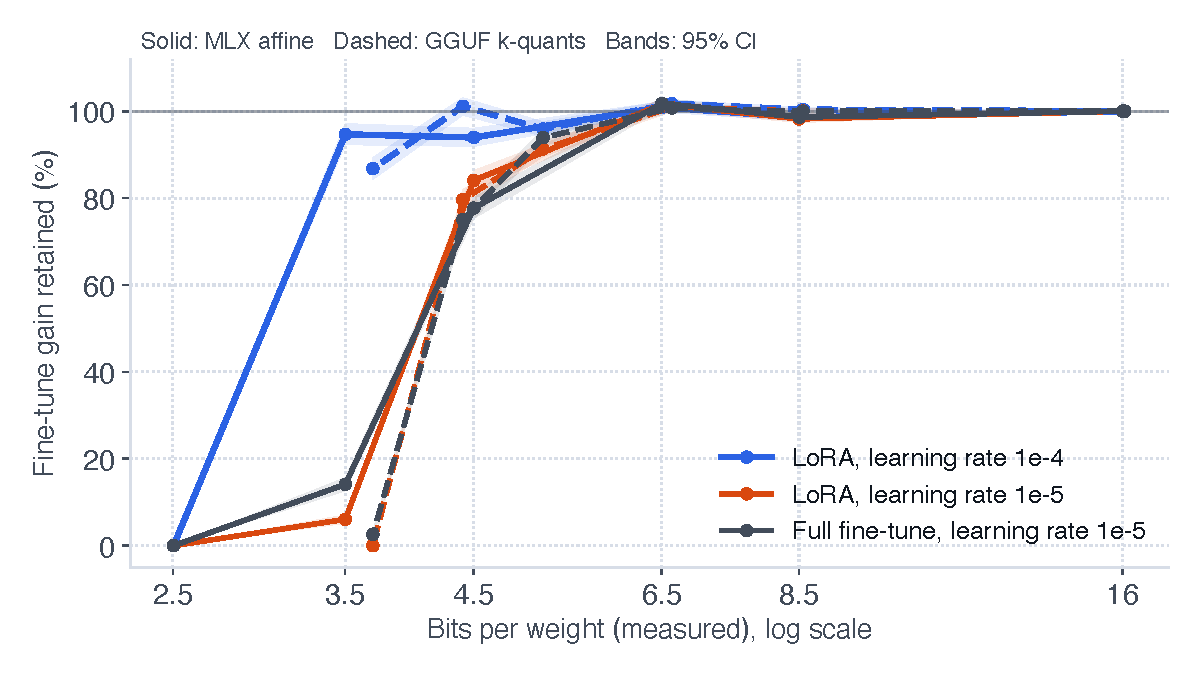
\includegraphics[width=0.64\linewidth]{figures/retention-q06.pdf}
\caption{Gain retained by three Qwen3-0.6B fine-tunes on banking77 against measured bits per weight (log scale; 16 is bf16): the LoRA at $10^{-4}$ (blue), the LoRA at $10^{-5}$ (orange) and full fine-tuning at $10^{-5}$ (dark gray). Solid lines: MLX affine; dashed: GGUF k-quants; bands: 95\% bootstrap intervals. The strong LoRA holds down to MLX~3-bit; the other two collapse there. Round 1, exploratory.}
\label{fig:retention}
\end{figure}

\subsection{Round 2: within a fine-tuning method, lower learning rates lost more}
\label{sec:lr}

Round 2 swept the learning rate on Qwen3-0.6B (Table~\ref{tab:lrsweep}; Figure~\ref{fig:lrsweep} in Appendix~\ref{app:extra}). Learning rate is the variable we manipulated; within each kind of fine-tuning, the update norm $\lVert\Delta\rVert$ grows with it. Within LoRA, the learning rate, the size of the update and whatever else a learning rate changes about the solution move together, so this design cannot say which of them matters; the title's ``small updates'' is shorthand for that bundle. Across kinds of fine-tuning, the norm does not order retention: full fine-tuning at $3\times10^{-5}$ ($\lVert\Delta\rVert = 18.6$) kept 0.78 of its gain at MLX~3-bit and 0.89 at Q2\_K, while LoRA at $3\times10^{-5}$ (25.2) kept 0.63 and 0.01. Gain retention was positively rank-correlated with learning rate in all eight combinations of fine-tuning kind and format we tracked at 3 and 4 bits: Spearman $\rho = 1.0$ in seven, and $0.8$ for LoRA at Q4\_K\_M, where $3\times10^{-5}$ and $10^{-4}$ are tied to within 0.001. Each combination has only three or four learning rates, so each is weak evidence alone. The bf16 accuracies did not rank the same way: the most accurate model at full precision, the LoRA at $10^{-5}$, kept 6\% of its gain at MLX~3-bit. A second seed moved $R$ at MLX~3-bit by at most 0.061 (0.95 and 0.92 for the LoRA at $10^{-4}$, 0.06 and 0.00 at $10^{-5}$), while bf16 accuracy moved by 8.4 and 3.5 points. On Qwen3-1.7B, the LoRA at $10^{-5}$ kept 36\% of its gain at MLX~3-bit and the LoRA at $10^{-4}$ kept 163\%. In accuracy retention, which the collapsing base does not inflate, the pair is 0.32 against 0.93.

\begin{table}[htbp]
\centering\small
\caption{Gain retention $R$ by learning rate, Qwen3-0.6B on banking77, seed 0 (round~2, exploratory). $\lVert\Delta\rVert$ is the norm of the update over all fine-tuned linear layers, measured after fusing in bf16. The LoRA at $3\times10^{-4}$ failed to learn and is omitted.}
\label{tab:lrsweep}
\begin{tabular}{llrrrrrrr}
\toprule
Kind & Learning rate & $\lVert\Delta\rVert$ & bf16 accuracy & MLX~4-bit & MLX~3-bit & Q4\_K\_M & Q3\_K\_M & Q2\_K \\
\midrule
\tablerows{tables/lrsweep.tex}
\bottomrule
\end{tabular}
\end{table}

\subsection{Weight-space correlates of retention}
\label{sec:mech-results}

This section is exploratory. Figure~\ref{fig:mechanism} in Appendix~\ref{app:extra} plots gain retention against NSR for the round-1 Qwen3-0.6B fine-tunes, and Table~\ref{tab:bands} counts all 89 fine-tune and format pairs from rounds 1 and 2. When the base is intact and most of the update survives, all 44 pairs with NSR below 3 kept at least 90\% of their gain, against 3 of 7 between 3 and 5 and 4 of 10 at 5 or more. The bands were chosen after looking at these data, so the table describes them and tests nothing. Within a fine-tuning method, NSR falls as the learning rate rises, so this association follows from the learning-rate effect itself and is not separate evidence for a mechanism.

The rounded-away mode is rare: five of 192 pairs. Full fine-tuning at $3\times10^{-6}$ produces an update so small, relative to the 3-bit quantization step, that the fine-tuned and base weights round to the same codes: only 5.5\% of its update's projection survives MLX~3-bit. Little noise is added because almost nothing is left, so its NSR (2.16) looks benign, and its measured gain retention is 0\%, although the base model also collapses there. At MLX~4-bit, where the base is intact, the same fine-tune keeps 50\% of its update and 27\% of its gain. Across rounds 1 to 4, the five pairs that kept less than 60\% of their update were all exploratory Qwen3-0.6B full fine-tunes, four of them from the run at $3\times10^{-6}$. No LoRA and no held-out fine-tune came close: the lowest update kept in rounds 3 and 4 was 74\%. In 168 of all 192 measured pairs, at least 98\% of the projection survived.

Base damage is a second axis. When the base model itself breaks, with base damage of 1 or more (for Qwen3-0.6B and Qwen3-1.7B: MLX~3-bit and 2-bit and GGUF~Q2\_K), only large updates held on: 4 of 24 such pairs kept 90\% of their gain. A large update can carry a broken base: at MLX~3-bit the Qwen3-0.6B base scored 0\%, while its LoRA at $10^{-4}$ kept 95\% of its gain. The noise ratio does not separate every case: at Q2\_K, the full fine-tune and the LoRA at $3\times10^{-5}$ (Section~\ref{sec:lr}) kept 89\% and 1\% of their gain with almost the same NSR (5.29 and 5.16). One untested explanation is that full fine-tuning also changes the RMSNorm weights, which neither format quantizes.

\subsection{Rounds 3 and 4: replication across family, task, seed and size}
\label{sec:replication}

Rounds 3 and 4 turned the round-2 observation into confirmatory tests. Each test asks whether the LoRA at $10^{-4}$ keeps more of its gain than the LoRA at $10^{-5}$, by a paired bootstrap of $R(10^{-4}) - R(10^{-5})$, at MLX~3-bit and at Q3\_K\_M. A test is supported only if its 95\% interval lies above zero. Round 3 moved to a new model family (OLMo-2 1B on banking77) and a new task (Qwen3-0.6B on MASSIVE); round~4 repeated both with a second seed and added Qwen3-4B. All 10 tests were supported (Table~\ref{tab:replication}), and all ten intervals also exclude zero at the Bonferroni-corrected level of 99.5\%. The tests are five fine-tune pairs at two correlated formats, and each interval describes one trained pair. The differences ranged from $+0.06$ (OLMo at Q3\_K\_M, with both seeds) to $+0.63$ (MASSIVE at MLX~3-bit, seed 1). Their sizes are not comparable across settings, because $R$ divides by each fine-tune's own gain, which is smaller for the strong LoRA, and a base that degrades therefore inflates the difference in the strong LoRA's favor. For Qwen3-4B at MLX~3-bit, 0.155 of the 0.539 difference comes from the base's own drop. The last column of Table~\ref{tab:replication} repeats each test on a quantity that does not involve the base: the gentle LoRA's accuracy drop minus the strong LoRA's (exploratory). It was positive in all ten, by 3.6 to 41.8 points, with every interval above zero.

\begin{table}[htbp]
\centering\footnotesize
\caption{The ten pre-registered tests of whether the LoRA at $10^{-4}$ keeps more of its gain than the LoRA at $10^{-5}$. Difference is $R(10^{-4}) - R(10^{-5})$ with a 95\% paired bootstrap interval. Drop is the accuracy lost by the LoRA at $10^{-5}$ minus that lost by the LoRA at $10^{-4}$, in points, with a 95\% interval; it does not involve the base and is exploratory. All ten tests were supported.}
\label{tab:replication}
\setlength{\tabcolsep}{4pt}
\begin{tabular}{llcrrll}
\toprule
Test & Setting & Format & $R$, $10^{-4}$ & $R$, $10^{-5}$ & Difference [95\% CI] & Drop [95\% CI] \\
\midrule
\tablerows{tables/replication.tex}
\bottomrule
\end{tabular}
\end{table}

Table~\ref{tab:pattern} shows accuracy retention for all eight settings in which both LoRAs were trained, including the three Qwen3 banking77 settings from rounds 1 and 2; Figure~\ref{fig:replication} in Appendix~\ref{app:extra} plots its 3-bit columns. In all eight, the gentle LoRA had the higher bf16 accuracy and kept less of its accuracy at each of the five formats compared (MLX~4-bit and 3-bit, GGUF~Q4\_K\_M, Q3\_K\_M and Q2\_K): 40 comparisons in the same direction. MLX~2-bit, evaluated only in round~1, left both Qwen3-0.6B LoRAs at 0\%. Two cautions apply. The eight settings are not independent, since three are second seeds of others. And at Q4\_K\_M the gaps are small: six of the eight are under 2 points, and for two of them, both on MASSIVE, the paired interval includes zero; for a third, OLMo-2 1B with seed 0, it excludes zero by less than $10^{-5}$. At MLX~4-bit every gap is at least 3.8 points, and at MLX~3-bit, Q3\_K\_M and Q2\_K at least 4.5.

Ranked by absolute accuracy, which is what a deployment ships, the answer depends on the format (Table~\ref{tab:absolute} in Appendix~\ref{app:extra}). The strong LoRA was the more accurate model at MLX~3-bit and Q2\_K in all eight settings and at Q3\_K\_M in seven, but only in five of eight at MLX~4-bit and in none at Q4\_K\_M, where the gentle LoRA's higher bf16 accuracy outweighed its larger loss. The strong LoRA's bf16 cost was 1.5 to 9.9 points.

Two checks argue against reading the gentle LoRAs as simply undertrained. Their final validation loss was no higher than the strong LoRAs' in any of the eight pairs. And the gap is not confined to items near a decision boundary: for Qwen3-4B at MLX~3-bit, among the test items each model answered correctly at bf16 with confidence of at least 0.9, the gentle LoRA still answered 89.6\% correctly after quantization and the strong LoRA 99.8\%. The gentle LoRAs' losses at 4 bits and at Q3\_K\_M were mostly wrong labels rather than broken outputs: the gentle Qwen3-0.6B LoRA produced a valid intent name for 99.3\% of items at MLX~4-bit and 99.5\% at Q3\_K\_M. Broken outputs were 43\% of its errors at MLX~3-bit and all of them at Q2\_K.

\begin{table}[htbp]
\centering\footnotesize
\caption{Accuracy retention $A$ at the five formats compared. Each cell gives the gentle LoRA ($10^{-5}$) / the strong LoRA ($10^{-4}$); the first column gives their bf16 accuracies in percent. Exploratory. $^\dagger$The 95\% paired interval of the gap includes zero.}
\label{tab:pattern}
\begin{tabular}{lcccccc}
\toprule
Setting & bf16 accuracy & MLX~4-bit & MLX~3-bit & Q4\_K\_M & Q3\_K\_M & Q2\_K \\
\midrule
\tablerows{tables/pattern.tex}
\bottomrule
\end{tabular}
\end{table}

Qwen3-4B differs in degree. Its base does not break at MLX~3-bit (base damage 0.64, against 1.21 for Qwen3-0.6B and 1.08 for 1.7B), and the gap between its two LoRAs is smaller there: accuracy retention 0.80 against 0.94, compared with 0.06 against 0.85 at 0.6B. At Q2\_K, where its base does break, the gentle 4B LoRA still loses 40\% of its accuracy. With one fine-tune pair per size, these numbers do not establish a trend with size.

Across seeds, OLMo reproduced closely: at MLX~3-bit and Q3\_K\_M, $R$ moved by at most 0.016 and bf16 accuracy by at most 1.5 points; at other formats $R$ moved by up to 0.042. MASSIVE did not. The direction held, but the gentle LoRA's gain retention at MLX~3-bit went from 0.32 with seed 0 to 0.05 with seed 1, and the strong LoRA's bf16 accuracy fell 7.7 points.

\subsection{Round 5: unrounded updates and training on the quantized base}
\label{sec:round5}

The weight-space account of Section~\ref{sec:mech-results} has a gap. In round~1 the gentle Qwen3-0.6B LoRA was also evaluated unfused, with its update kept exactly in bf16 on top of the quantized base, and it lost about as much as the fused model: $R$ was 0.83 unfused against 0.84 fused at MLX~4-bit, and 0.02 against 0.06 at 3-bit, where that base collapses. An update that is never quantized cannot be rounded away. These exploratory runs, which our first draft did not report, point to a different account: a small update stops working when quantization moves the weights it was trained against by more than the update itself, whether or not the update is quantized. Round~5 tested that account and the remedy it implies, under a plan pushed to a hosted repository before anything ran (Table~\ref{tab:round5}). A 20-item plumbing test ran after the plan was hashed; its numbers were not used.

W5-H1 asked whether an update that is never rounded rescues a gentle fine-tune. We tested it on OLMo-2 1B at MLX~3-bit, where the base stays usable (14.5\% at bf16, 6.8\% at 3-bit) while the fused gentle LoRAs kept only 0.83 and 0.81 of their gain. If rounding of the update caused the loss, unfusing should recover most of the missing 0.17 to 0.19; the plan called the hypothesis supported if each seed's upper bound stayed below $+0.08$. Unfusing changed $R$ by $+0.008$ [$-0.010$, $+0.027$] for seed~0 and $+0.023$ [$+0.002$, $+0.042$] for seed~1, so W5-H1 was supported: the unrounded update recovered 5\% and 12\% of the loss by point estimate, and 16\% and 22\% at the upper ends of the intervals. The strong LoRAs, and both kinds at MLX~4-bit, behaved the same way, with unfused and fused models within 0.015 of each other in $R$ (exploratory).

W5-H2 asked whether training against the shipped base removes the loss. A gentle LoRA trained by mlx-lm directly on the 4-bit Qwen3-0.6B base, the QLoRA setup, and evaluated unfused on that base delivered 96\% of the bf16 gain, against 84\% for the same LoRA trained in bf16, fused and quantized: a difference of $+0.116$ [$+0.097$, $+0.135$], so W5-H2 was supported. Its accuracy at 4 bits, 77.6\%, was within a point of what the bf16-trained LoRA reached at bf16 (78.5\%), and its final validation loss was nearly the same (0.057 against 0.056). The exploratory runs qualify the remedy. On the 3-bit base, which scores 0\% on its own, a gentle LoRA trained there reached 67.5\% and delivered 95\% of the bf16 gain, against 6\% for the fuse-then-quantize one (a difference of $+0.890$ [$+0.865$, $+0.916$]), although its final validation loss was higher than in bf16 (0.099 against 0.056). At the strong learning rate, training on the quantized base did not help: the strong LoRA trained less well there (final validation loss 0.110 at 4 bits and 0.121 at 3 bits, against 0.067 in bf16) and delivered 78\% of the gain at 4 bits and 94\% at 3 bits, against 94\% and 95\% when trained in bf16, fused and quantized: differences of $-0.158$ [$-0.181$, $-0.136$] and $-0.007$ [$-0.032$, $+0.018$]. The most accurate 4-bit and 3-bit models in this comparison were the gentle LoRAs trained on the quantized base.

Two further checks bear on the earlier rounds. Rebuilt from the round-1 adapter, the gentle LoRA's Q3\_K\_M file scored 62.1\% with four llama-server slots and with one; the two runs differed on 2 of 3,080 items, and each differed from the round-1 run on 3. And restricting decoding to the 77 intent names changed accuracy retention by at most 0.003 (the gentle LoRA at Q3\_K\_M kept 0.793 of its accuracy with the restriction and 0.791 without; the strong one 0.987 and 0.985), so the gentle LoRA's losses there are wrong labels, not broken outputs. At Q2\_K it kept 2\% of its accuracy even when forced to name a valid intent.

\begin{table}[htbp]
\centering\footnotesize
\caption{Round~5. Top: $R$ of OLMo-2 1B LoRAs at MLX~3-bit, fused and quantized against unfused on the quantized base. Bottom: share of the bf16 gain delivered at the training format by a Qwen3-0.6B LoRA trained on the quantized base ($S$), against $R$ of the same LoRA trained in bf16, fused and quantized. Differences are paired bootstrap 95\% intervals. W5-H1 needed each upper bound below $+0.08$ and W5-H2 an interval above zero; both were supported.}
\label{tab:round5}
\begin{tabular}{lllll}
\toprule
Test & LoRA & Format & Two pipelines & Difference [95\% CI] \\
\midrule
\tablerows{tables/round5.tex}
\bottomrule
\end{tabular}
\end{table}

In these MLX tests (OLMo-2 1B at 3 bits, Qwen3-0.6B at 4 bits, banking77), the loss followed the base rather than the update. A gentle update trained against the bf16 weights did not survive their move to the quantized grid, even when the update itself was kept exact, while a gentle LoRA trained against the quantized weights did. The weight measurements of Section~\ref{sec:mech-results} fit this reading if NSR is taken as the size of the quantization step relative to the update, which is what it tracks; they do not show that the update's own rounding matters. For gentle LoRAs, the remedy is the one QLoRA builds in by training on the quantized base \citep{dettmers2023qlora}, and that LoftQ prepares for at initialization \citep{li2023loftq}: train against the weights that will ship. GGUF has no such training path in our pipeline and was not tested.

\subsection{Predicting retention before quantizing}
\label{sec:predictor}

Round 2 tested whether the weight measurements predict gain retention without evaluating the quantized fine-tune. Predictor v1, a logistic model of NSR and base damage fitted on the round-1 Qwen3-0.6B points and frozen, met two of its three pre-registered criteria and missed the third, a mean absolute error (MAE) of at most 0.10 on new learning rates and seeds, by 0.007 (Appendix~\ref{app:predictor}); as pre-registered, the tool was then limited to descriptive output. Its largest miss was the full fine-tune at $3\times10^{-6}$ at MLX~3-bit, whose update is rounded away: NSR measures only the noise, so it read a vanished update as safe. Predictor v2 adds update kept,
\begin{equation}
\hat R = \sigma\left(5.612 + 3.296 \ln \frac{\mathrm{kept}}{\mathrm{NSR}} - 1.555 \ln \mathrm{KLD}_{\mathrm{base}}\right),
\end{equation}
with its form chosen among four candidates by leave-one-fine-tune-out cross-validation on all 89 round-1 and round-2 points (error 0.071, against 0.095 for the v1 form), and was frozen before round~3.

Predictor v2 passed both of its pre-registered tests in rounds 3 and 4 (Table~\ref{tab:baselines}; Figure~\ref{fig:predictor} in Appendix~\ref{app:predictor}): an accuracy bar, MAE at most 0.10 with agreement on the call ``keeps at least 90\%'' of at least 0.85 (W3-H2, W4-H3), and a lower MAE than two baselines, the mean retention of each format and a one-feature model of base damage (W3-H3, W4-H4). Its MAE was 0.059 on round~3 (OLMo-2 1B and MASSIVE, 35 points) and 0.084 on round~4 (second seeds and Qwen3-4B, 42 points), where the interval reaches 0.146, above the bar, and overlaps the base-damage baseline's. Predictor v1 would also have met the accuracy bar in both rounds (0.071 and 0.090). With five or six held-out fine-tunes per round the bars cannot separate the two versions, and no held-out fine-tune entered the rounded-away regime that update kept was added for: the lowest update kept was 74\% in round~3 and 98.5\% in round~4.

Two baselines that were not pre-registered put these errors in context (Table~\ref{tab:baselines}). Predicting full retention everywhere, $\hat R = 1$, scores 0.153 in round~3, where v2 beats it by 0.094 [0.003, 0.188] (paired, resampling fine-tunes), but 0.102 in round~4, where the difference, 0.019, has an interval from $-0.076$ to 0.127. A model of the update's norm and base damage, $\sigma(a + b \ln \lVert\Delta\rVert + c \ln \mathrm{KLD}_{\mathrm{base}})$, fitted by the same procedure on the same 89 points, does better than v2: its leave-one-fine-tune-out error is 0.061 against 0.071, its held-out error is 0.049 in both rounds, and in round~4 it beats v2 by 0.035 [0.006, 0.070]. Over the 89 fitting points, $\ln \mathrm{NSR}$ and $\ln \lVert\Delta\rVert$ correlate at $-0.83$ to $-0.97$ within nine of the ten formats ($-0.55$ at MLX~3-bit; three formats have only four points). So the weight-space measurements have not been shown to add information beyond the size of the update.

\begin{table}[htbp]
\centering\footnotesize
\caption{Held-out error of the predictors and baselines in rounds 3 and 4: MAE against $R$ clipped to $[0,1]$, with 95\% intervals from resampling whole fine-tunes, and safe-call agreement. The last two rows were added after the pre-registered tests and are exploratory; the update-norm model was fitted by the same procedure and on the same 89 points as v2.}
\label{tab:baselines}
\begin{tabular}{lllll}
\toprule
& \multicolumn{2}{l}{Round 3 (35 points)} & \multicolumn{2}{l}{Round 4 (42 points)} \\
Model & MAE [95\% CI] & Safe & MAE [95\% CI] & Safe \\
\midrule
\tablerows{tables/baselines.tex}
\bottomrule
\end{tabular}
\end{table}

The misses follow two patterns. On MASSIVE, when the base breaks, the slot-annotation task loses more than a small noise ratio suggests: the LoRA at $10^{-4}$ at MLX~3-bit was predicted to keep 98\% of its gain and kept 62\% (seed 0) and 69\% (seed 1). On banking77, the OLMo and Qwen3-4B fine-tunes kept more than a large noise ratio suggests: the gentle 4B LoRA kept 92\% of its gain at MLX~3-bit with NSR 6.85, where v2 predicted 48\%. At Q2\_K the same model has $R = 1.28$ against a prediction of 5\%, but only because its base collapsed; the fine-tune itself kept 60\% of its accuracy. On the 14 Qwen3-4B points alone, v2's MAE was 0.115 and its agreement 0.79, short of both bars. That breakdown was not pre-registered. After seeing it, we decided that \texttt{ftquant check} would not predict for Qwen3-4B. Seed-to-seed variation is also invisible to the weights: the two MASSIVE seeds of the gentle LoRA had almost identical measurements and the same 41\% prediction at MLX~3-bit, but kept 32\% and 5\% of their gain.

\subsection{Operating-point drift (exploratory)}
\label{sec:drift}

The one pre-registered test of operating-point drift, round-1 H4 at 4 bits, was not supported, because GGUF~Q4\_K\_M moved coverage by only 1.2 points. At lower bit widths, coverage fell much more than accuracy. For the round-1 Qwen3-1.7B LoRA, MLX~3-bit kept 93\% of the accuracy but cut the share of auto-accepted items from 38.1\% to 27.8\%, and Q2\_K kept 85\% of the accuracy but cut coverage from 36.4\% to 10.1\%. Across the eight settings and five formats of Table~\ref{tab:pattern}, the gentle LoRA's coverage fell further than the strong LoRA's in 36 of 40 cases; the exceptions are Qwen3-1.7B at Q4\_K\_M and the second MASSIVE seed at MLX~3-bit, Q4\_K\_M and Q2\_K. At MLX~4-bit, the Qwen3-0.6B LoRA at $10^{-5}$ kept 88.5\% of its accuracy but accepted 19.4 points fewer items. The items a gentle LoRA still accepted were also less reliable: at MLX~3-bit its error among accepted items rose from 5.1\% to 12.8\% on Qwen3-4B, from 3.8\% to 11.4\% on OLMo-2 1B (seed 0) and from 5.4\% to 23.2\% on Qwen3-1.7B, while the strong LoRAs ended at 4.9\% to 5.5\%. These are point estimates on the half of the test set not used to fit $\tau$; a system that sends low-confidence outputs to a person would see its workload change at formats where accuracy still looks acceptable. This fits the finding that quantization lowers confidence most on items a model was unsure of \citep{proskurina2024confidence}, and is a single-threshold counterpart of what \citet{zhu2026conformal} report for conformal prediction under configuration shift.

\section{Limitations}
\label{sec:limits}

\begin{itemize}
\item \textbf{Scale and tasks.} Four base models, none larger than 4B, and only Qwen3-4B above 1.7B, with one seed. Two tasks, both with short outputs scored by exact match; long-form generation may degrade differently.
\item \textbf{Fine-tuning.} LoRA rank 8 and scale 20 only, 500 steps (about a fifth of an epoch), and the same nominal learning rates at every size. ``Gentle'' names a learning rate at one LoRA scale, not an update size. The 4B fine-tunes' gains are small (27 points for the gentle LoRA and 21 for the strong), so their $R$ values are noisier. Full fine-tuning was run only on Qwen3-0.6B, with one seed.
\item \textbf{Round 5.} banking77 only; the unfused test on OLMo-2 1B at MLX~3-bit, and training on the quantized base on Qwen3-0.6B in MLX with one seed; no GGUF counterpart.
\item \textbf{Formats.} MLX group size 64 only, GGUF without an importance matrix, and no calibration-based methods such as GPTQ or AWQ; an importance matrix may shrink the losses at Q3\_K\_M and Q2\_K.
\item \textbf{Metrics and uncertainty.} $R$ exceeds 1 whenever the base loses more than the fine-tune, which makes it hard to read at 3 bits and below, so we report accuracy retention next to it. Bootstrap intervals cover test-set sampling only, and seed-to-seed variation can be larger (Section~\ref{sec:replication}). $\tau$ was fitted on half of the test set rather than the planned validation split, and the drift numbers are point estimates.
\item \textbf{Predictor.} Its round-4 interval crosses the 0.10 bar, it fails on the 4B subgroup, and a post hoc model of update size and base damage did as well or better. Its added input, update kept, targets a failure mode that no held-out fine-tune reached, and its reading bands were chosen post hoc.
\item \textbf{Process.} The pre-registrations were not reviewed externally, their timestamps are self-recorded except for the pushes of rounds 3 to 5, and all runs used one machine. Round~5 was designed after we had seen the round-1 unfused results that motivated it.
\end{itemize}

\section{Conclusion}
\label{sec:conclusion}

At MLX~3-bit and GGUF~Q3\_K\_M, the gentle LoRA kept less of its gain than the strong one in 10 of 10 pre-registered tests across three base models and two tasks (F1), and it kept a smaller share of its accuracy at all five formats compared, 40 of 40 (F2). In MLX, the loss did not come from rounding the update: the exact update recovered 5\% and 12\% of it, with upper 95\% bounds of 16\% and 22\% (F4), while training the gentle LoRA on the quantized base delivered 96\% of its bf16 gain at 4 bits, against 84\% (F5). The weight measurements describe these losses but have not been shown to predict them better than the size of the update (F6). In practice, select a fine-tune on the quantized artifact it will ship as: the gentle LoRA was the more accurate model at Q4\_K\_M in all eight settings, the strong one at MLX~3-bit and Q2\_K in all eight and at Q3\_K\_M in seven (F3). Keeping the adapter unfused does not rescue a gentle LoRA in MLX; training it on the quantized base does, and gave our most accurate 4-bit and 3-bit models, but it cost the strong LoRA 0.158 of $R$ at 4 bits and was not tested for GGUF.

\subsubsection*{Broader Impact Statement}
This work measures how quantization changes fine-tuned models that people already ship, and describes a check that flags risky formats before deployment. The main risk is overtrust: the predictor was tested only on the models, tasks and formats listed here, so the tool prints no prediction outside that scope. All data sets and models used are publicly available.

\bibliography{refs}
\bibliographystyle{tmlr}

\appendix

\section{Pre-registration record}
\label{app:deviations}

Table~\ref{tab:protocol} lists the five rounds, when each plan was hashed and what it found; Table~\ref{tab:deviations} lists every deviation from the plans.

\begin{table}[htbp]
\centering\small
\caption{The five pre-registered rounds. Plan hashed: the time (PDT) at which each plan's hash was recorded.}
\label{tab:protocol}
\begin{tabularx}{\linewidth}{clLl}
\toprule
Round & Plan hashed & Confirmatory question & Outcome \\
\midrule
1 & 27 Sep 17:39 & How much of a LoRA's gain survives each format on Qwen3-1.7B? & H1 supported; H2, H4 not; H3 inconclusive \\
2 & 27 Sep 18:00 & Does predictor v1 predict retention on new fine-tunes? & P2, P3 met; P1 not met \\
3 & 28 Sep 08:40 & Do small updates lose more on a new family and task? Does predictor v2 pass? & W3-H1 to W3-H3 supported \\
4 & 28 Sep 18:11 & Do the results hold for second seeds and Qwen3-4B, with v2 unchanged? & W4-H1 to W4-H4 supported \\
5 & 3 Oct 19:49 & Does an unrounded update rescue a gentle LoRA? Does training on the quantized base? & W5-H1, W5-H2 supported \\
\bottomrule
\end{tabularx}
\end{table}

\begin{table}[h]
\centering\footnotesize
\caption{Deviations from the pre-registered plans, in time order.}
\label{tab:deviations}
\begin{tabularx}{\linewidth}{llLL}
\toprule
When (PDT) & Round & Deviation & Effect \\
\midrule
27 Sep, 18:00 & 1 & The analysis code for $\tau$ was changed to match the written definition, before any 1.7B result existed. & None on confirmatory results. \\
27 Sep, 23:48 & 2 & The predictor freeze step crashed on a missing folder before writing anything, and was re-run. & None. \\
28 Sep, 08:29 & 2 & LoRA at $3\times10^{-4}$ failed to learn, so its $R$ is undefined; its 7 points were excluded from the round-2 test on new learning rates and seeds (P1, P2). & That test was scored on 42 points instead of 49 (Table~\ref{tab:predictor}). \\
29 Sep, 05:16 & 4 & The 4B fine-tunes ran out of memory at batch size 4 and were trained with micro-batches of 2 and two-step accumulation. & Same effective batch, steps and examples. \\
29 Sep, 16:29 & 2 to 4 & $\tau$ was fitted on half of the test set, not the validation split the round-1 plan named for later rounds. Found in an audit. & Exploratory drift numbers only. \\
4 Oct, 00:55 & 5 & The exploratory run training the LoRA at $10^{-4}$ on the 3-bit base slowed sharply under memory pressure after its step-100 checkpoint; it was stopped after step 200 and retrained from scratch with the same settings. & None on the confirmatory results. \\
\bottomrule
\end{tabularx}
\end{table}

\clearpage
\section{Additional results}
\label{app:extra}

\begin{table}[tb]
\centering\small
\caption{Gain retention by measurement band, over the 89 fine-tune and format pairs of rounds 1 and 2 (Qwen3-0.6B and Qwen3-1.7B on banking77). The bands were chosen after seeing these data.}
\label{tab:bands}
\begin{tabular}{lrrr}
\toprule
Measurement & Pairs & Kept $\ge 90\%$ of gain & Lowest \\
\midrule
\tablerows{tables/bands.tex}
\bottomrule
\end{tabular}
\end{table}

\begin{table}[htbp]
\centering\small
\caption{Base models and tasks. Base accuracy is zero-shot, at bf16 in MLX, on the full test set. All fine-tunes run 500 optimizer steps at an effective batch size of 4.}
\label{tab:bases}
\begin{tabularx}{\linewidth}{llcrL}
\toprule
Base model & Task & Rounds & Base accuracy & Fine-tunes (learning rates) \\
\midrule
\tablerows{tables/bases.tex}
\bottomrule
\end{tabularx}
\end{table}

\begin{table}[htbp]
\centering\footnotesize
\caption{Round-1 confirmatory hypotheses: Qwen3-1.7B LoRA at $10^{-4}$ on banking77. Values are $R$ unless stated; brackets are 95\% paired bootstrap intervals.}
\label{tab:week1}
\begin{tabularx}{\linewidth}{l>{\raggedright\arraybackslash}p{3.6cm}Ll}
\toprule
& Pre-registered criterion & Result & Verdict \\
\midrule
\tablerows{tables/week1.tex}
\bottomrule
\end{tabularx}
\end{table}

\begin{figure}[tb]
\centering
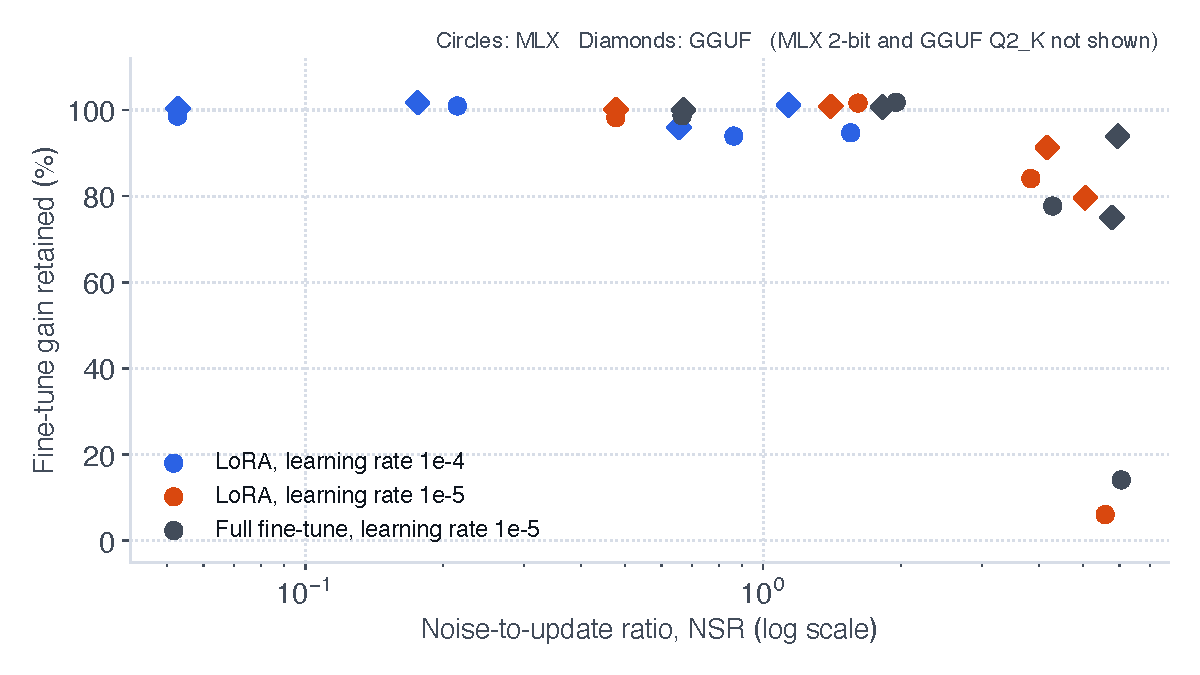
\includegraphics[width=0.84\linewidth]{figures/mechanism-q06.pdf}
\caption{Gain retained against the noise-to-update ratio NSR (log scale) for the round-1 Qwen3-0.6B fine-tunes, at every format except MLX~2-bit and GGUF~Q2\_K. The base model also breaks at MLX~3-bit; the two points at the lower right are the gentle LoRA and the full fine-tune there. Circles: MLX; diamonds: GGUF.}
\label{fig:mechanism}
\end{figure}

\begin{figure}[htbp]
\centering
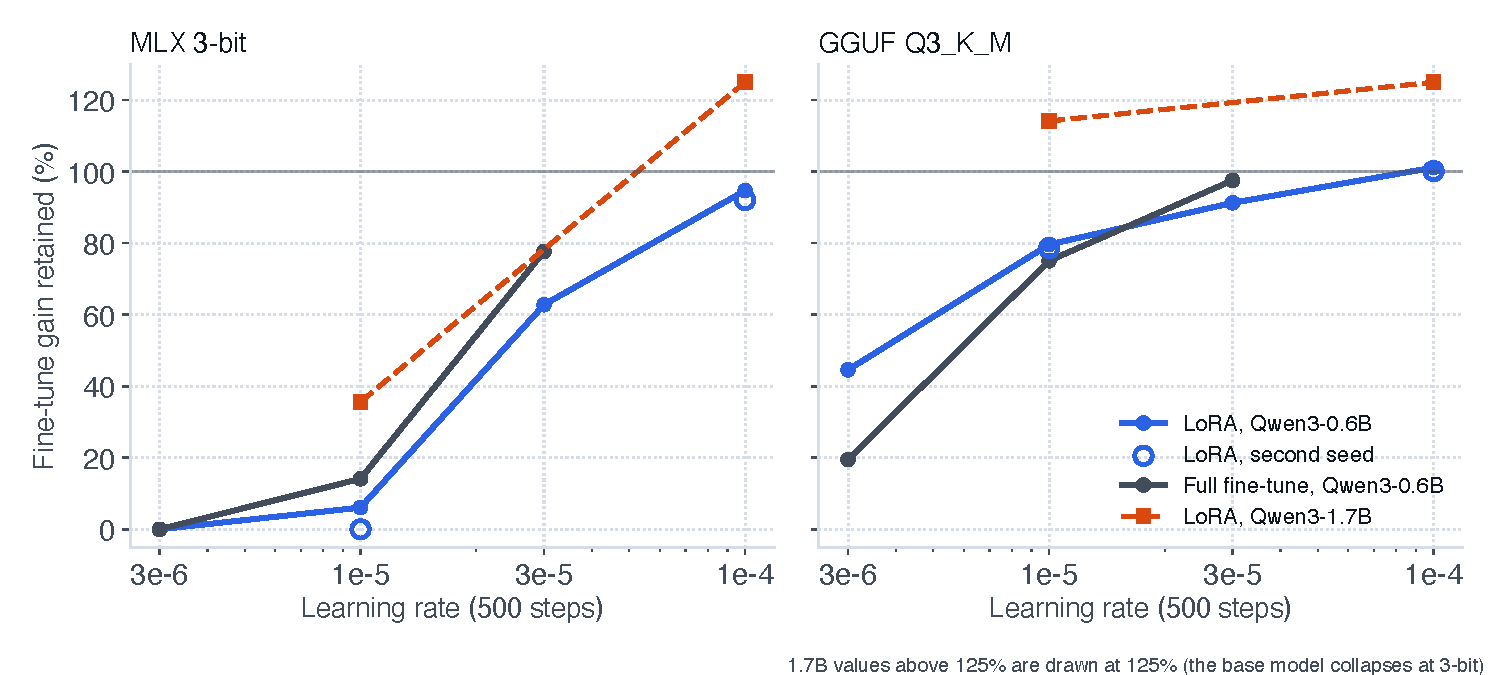
\includegraphics[width=\linewidth]{figures/lr-sweep.pdf}
\caption{Gain retained at MLX~3-bit and GGUF~Q3\_K\_M against learning rate. Qwen3-1.7B values above 125\% are drawn at 125\%, because its base collapses at 3 bits. Round 2, exploratory.}
\label{fig:lrsweep}
\end{figure}

\begin{table}[htbp]
\centering\small
\caption{Quantization formats and bits per weight (bpw) measured from the files. MLX files were measured for Qwen3-0.6B only; group-64 affine quantization stores a 16-bit scale and bias for every 64 weights, which adds 0.5 bits per weight at any model size.}
\label{tab:formats}
\begin{tabular}{llrrl}
\toprule
Engine and format family & Format & bpw, Qwen3-0.6B & bpw, Qwen3-1.7B & Rounds \\
\midrule
\tablerows{tables/formats.tex}
\bottomrule
\end{tabular}
\end{table}

\begin{figure}[htbp]
\centering
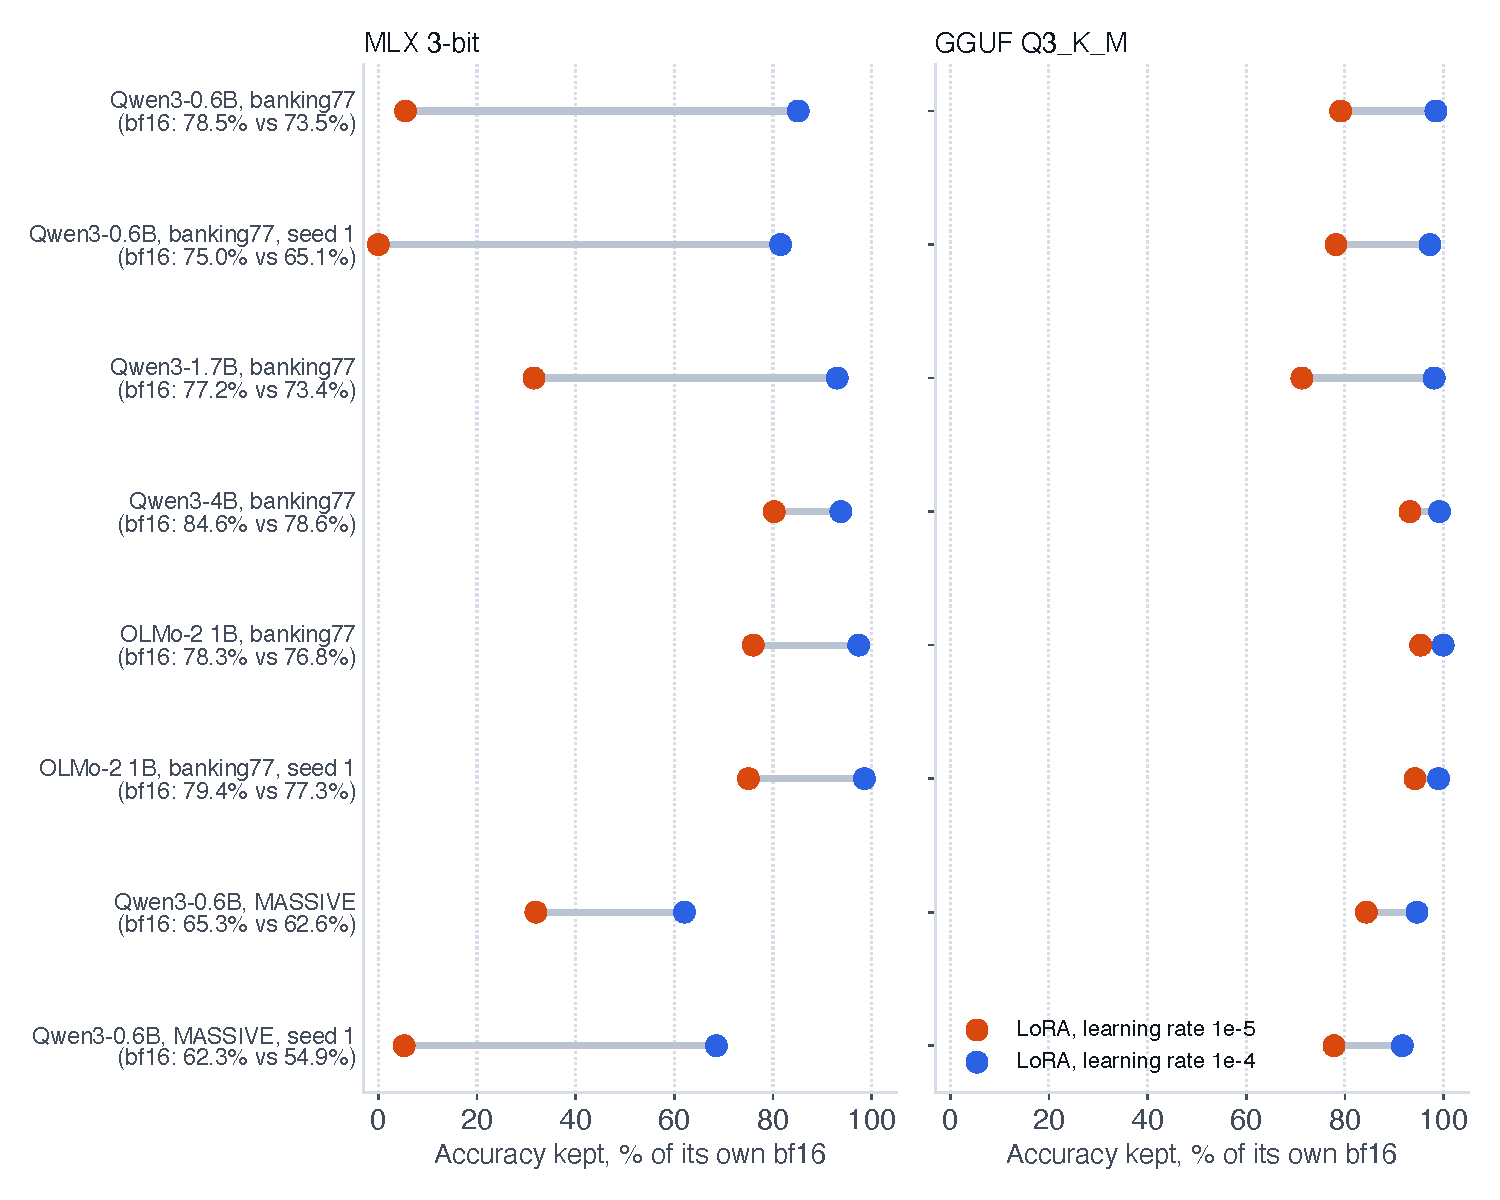
\includegraphics[width=0.86\linewidth]{figures/replication.pdf}
\caption{Accuracy kept, as a share of each model's own bf16 accuracy, by the LoRA at $10^{-5}$ (orange) and the LoRA at $10^{-4}$ (blue), at MLX~3-bit and GGUF~Q3\_K\_M, in all eight settings. Labels give the two bf16 accuracies. Exploratory.}
\label{fig:replication}
\end{figure}

\begin{table}[htbp]
\centering\footnotesize
\caption{Absolute accuracy in percent: the gentle LoRA ($10^{-5}$) / the strong LoRA ($10^{-4}$), with the more accurate model in bold at each quantized format. The bf16 column is MLX. Exploratory.}
\label{tab:absolute}
\setlength{\tabcolsep}{4pt}
\begin{tabular}{lcccccc}
\toprule
Setting & bf16 & MLX~4-bit & MLX~3-bit & Q4\_K\_M & Q3\_K\_M & Q2\_K \\
\midrule
\tablerows{tables/absolute.tex}
\bottomrule
\end{tabular}
\end{table}

\clearpage
\section{Predictor details}
\label{app:predictor}

Predictor v1 was fitted by least squares against $R$ clipped to $[0,1]$, on the round-1 Qwen3-0.6B points only, and frozen:
\begin{equation}
\hat R = \sigma\left(8.707 - 5.81 \ln \mathrm{NSR} - 2.794 \ln \mathrm{KLD}_{\mathrm{base}}\right).
\end{equation}
Its test had three pre-registered criteria. On new learning rates and seeds, its MAE had to be at most 0.10, and its agreement with the measurements on the call ``keeps at least 90\%'' at least 0.85 (P1). It had to beat two baselines: the mean retention of each format (bits-only) and a one-feature model of base damage (KLD-only) (P2). On Qwen3-1.7B, its MAE had to be at most 0.15 and its agreement at least 0.80 (P3). P2 and P3 were met; P1 was not, by 0.007, inside an interval from 0.048 to 0.182 (Table~\ref{tab:predictor}). In rounds 3 and 4, v1 did almost as well as v2 (0.090 against 0.084 in round~4), and better on round~4's MASSIVE arm (0.072 against 0.088; in round~3, 0.073 against 0.063). Without the easy 6-bit formats, v2's round-4 error was 0.115, against 0.080 in round~3.

\begin{table}[htbp]
\centering\footnotesize
\caption{Pre-registered predictor tests. MAE is against $R$ clipped to $[0,1]$, with 95\% intervals from resampling whole fine-tunes. Safe is the share of points where predicted and measured retention fall on the same side of 0.9. The two baseline columns give the MAE of the pre-registered baselines, fitted on the same points as the predictor; their intervals are in Table~\ref{tab:baselines}. W3-H2 and W4-H3 are the accuracy bars; W3-H3 and W4-H4 require beating both baselines. $^\ast$Exploratory breakdown of 2 fine-tunes, without an interval.}
\label{tab:predictor}
\begin{tabularx}{\linewidth}{Lrlcccl}
\toprule
Test & $n$ & MAE [95\% CI] & Safe & MAE, KLD-only & MAE, bits-only & Result \\
\midrule
\tablerows{tables/predictor.tex}
\bottomrule
\end{tabularx}
\end{table}

\begin{figure}[htbp]
\centering
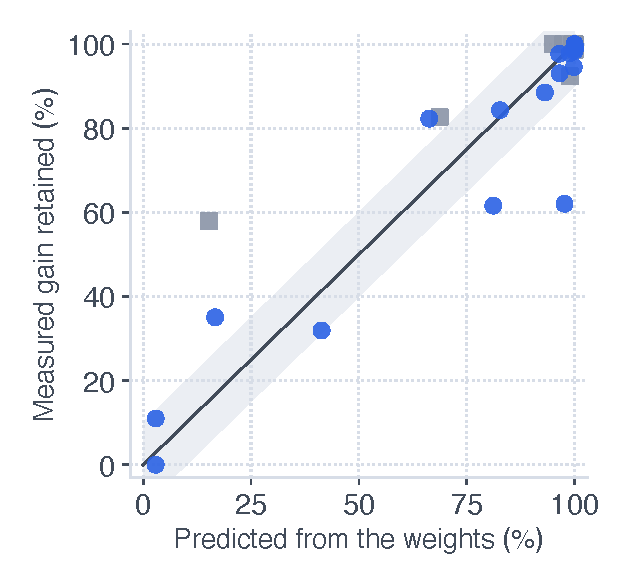
\includegraphics[width=0.49\linewidth]{figures/predictor-v2-week3.pdf}\hfill
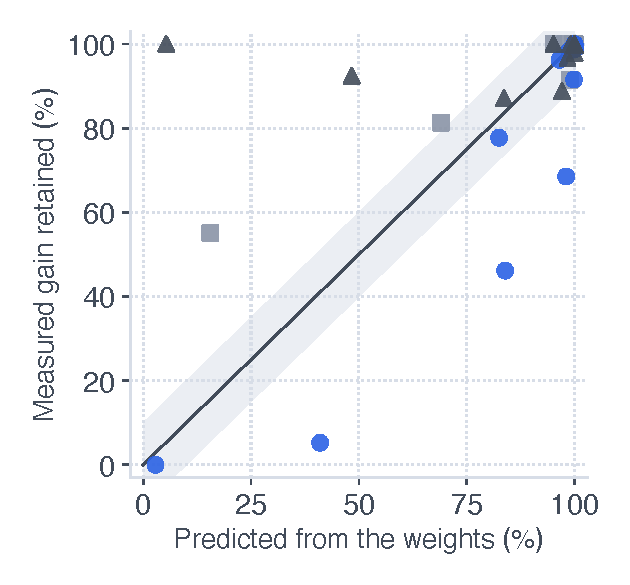
\includegraphics[width=0.49\linewidth]{figures/predictor-v2-week4.pdf}
\caption{Predictor v2's predictions, made from the weights without evaluating the quantized models, against measured gain retention (capped at 100\%). Left: round~3, 35 points (squares: OLMo-2 1B on banking77; circles: Qwen3-0.6B on MASSIVE). Right: round~4, 42 points (squares: OLMo-2 1B, seed 1; circles: Qwen3-0.6B on MASSIVE, seed 1; triangles: Qwen3-4B on banking77). The band marks $\pm 10$ points.}
\label{fig:predictor}
\end{figure}

\clearpage
\section{Every fine-tune}
\label{app:runs}

Table~\ref{tab:grid} lists the 23 fine-tunes of rounds 1 to 4, including the run that failed to learn. Together with the base models they account for 279 full-test-set evaluations. $\lVert\Delta\rVert$ is the norm of the update over all fine-tuned linear layers, measured on the bf16 fused weights; for round~4 it was computed from the adapters with the same procedure, which reproduces the recorded round-3 values to within 0.2\%.

\begin{table}[htbp]
\centering\footnotesize
\caption{The fine-tunes of rounds 1 to 4. Accuracy is at bf16 in MLX. Evaluations counts the full-test-set evaluations, including bf16 in both engines and, in round~1, three unfused-adapter runs.}
\label{tab:grid}
\begin{tabular}{clllllrrrl}
\toprule
Round & Base model & Task & Kind & Learning rate & Seed & Accuracy & $\lVert\Delta\rVert$ & Evaluations & Note \\
\midrule
\tablerows{tables/grid.tex}
\bottomrule
\end{tabular}
\end{table}

\clearpage
\section{The \texttt{ftquant check} tool}
\label{app:tool}\label{sec:tool}

\texttt{ftquant check} implements Section~\ref{sec:mechanism} for a user's own fine-tune. It reads an MLX or PEFT adapter, or a full checkpoint, streams the safetensors, and runs the exact quantizer on the base and fine-tuned weights. It prints update kept, NSR and base damage. It adds v2's prediction only where v2 was tested: MLX 6, 4 and 3-bit with group size 64 and GGUF~Q6\_K, Q4\_K\_M, Q3\_K\_M and Q2\_K, on the three bases whose base damage ships with the tool (Qwen3-0.6B, Qwen3-1.7B and OLMo-2 1B). v2 was fitted on Qwen3-0.6B and Qwen3-1.7B banking77 fine-tunes and tested on held-out OLMo-2 1B, Qwen3-0.6B MASSIVE and Qwen3-4B fine-tunes. The tool needs only numpy. For a Qwen3-0.6B LoRA trained on MASSIVE at $10^{-5}$, a fine-tune v2 had never seen, it printed:

\begin{scriptsize}
\begin{verbatim}
format                     noise/update  update kept  base damage  predicted gain kept  reading
MLX 8-bit (group 64)               0.47         100%        0.004                  n/a  low noise
MLX 6-bit (group 64)               1.59         100%        0.021                 100%  low noise
MLX 4-bit (group 64)               3.80         100%        0.255                  97%  moderate noise
MLX 3-bit (group 64)               5.52          99%        1.207                  41%  high noise, base model breaks
\end{verbatim}
\end{scriptsize}

\noindent Measured on its 2,974 test items, that fine-tune kept 93\% of its gain at MLX~4-bit and 32\% at 3-bit. The reading column uses the bands of Table~\ref{tab:bands}. The seed-1 run of the same configuration had the same prediction and kept 5\% (Section~\ref{sec:predictor}).

\section{Reproducibility and compute}
\label{app:repro}

Software: MLX 0.32.2 and mlx-lm 0.31.3; llama.cpp build 11146 (commit 7fe450e19), whose \texttt{gguf-py} and converter are vendored at the same commit. Data: PolyAI's banking77 CSV files and Amazon's MASSIVE release, both checked against recorded SHA-256 hashes by the fetch script. \Suppname{} holds the five pre-registrations and their hash logs, the frozen predictors (v1 SHA-256 prefix \texttt{5df7d620}, v2 \texttt{6fd78627}), the per-item predictions of every evaluation, every training configuration and log, and a lab notebook written as the runs happened. Its README maps every table and figure in this paper to the script and the result files that produce it, and \texttt{python -m ftquant.findings} recomputes every number quoted in the text, with the source of each, into \texttt{runs/findings/findings.json}; repeated runs produce identical files. Re-scoring all results from the per-item predictions needs only Python with numpy and PyYAML.

Everything ran on one Apple M1 Pro laptop with 16 GB of memory: rounds 1 to 4 in 51.4 hours of wall-clock time from the first sweep (27 September, 12:45) to the last verdicts (29 September, 16:12), and round~5 in 14.5 hours from 3 October, 20:03, to 4 October, 10:33, several steps of which were slowed by memory pressure on the shared laptop (Appendix~\ref{app:deviations}). In rounds 1 to 4, a LoRA run of 500 steps took 10.2 to 19.8 minutes on Qwen3-0.6B, 52.3 to 55.8 on 1.7B, 40.5 to 52.8 on OLMo-2 1B and 127.8 to 143.8 on 4B. One full-test-set evaluation took 2.3 to 22.7 minutes on the smaller models and 12.0 to 25.2 on 4B, and the round-4 mechanism measurements for two fine-tunes took 4.5 to 8.1 minutes on the 0.6B and 1B models and 29.6 on 4B. In round~5, three of the four LoRA runs on a quantized Qwen3-0.6B base took 27.9 to 28.3 minutes; the fourth, retrained after it stalled, took 223.8 minutes of wall-clock time.

\end{document}
